\chapter{Background and Related Work}
%\section{Section1}
This thesis is an attempt to apply the theoretical \unsure{How to write acronyms}{\gls{ddmpc}} developed by Xie in \cite{xie2024}. The considered application is a model-scale bicycle at the \gls{IST}, University of Stuttgart. The bicycle was chosen as the \gls{IST} has a rear-steered bicycle which is a more complex system that could be tested against the results achieved from this project. In the following sections, the bicycle modelling and Data-driven MPC are discussed.

\section{Bicycle Modelling}

The first step towards the design of the controllers that will balance and smooth the motion is to model the bicycle. Bicycles are nonlinear and unstable, and therefore developing mathematical models with high accuracy has been an important area of research in recent times. Bicycle dynamics have been modeled using many techniques, including state-space models, kinetic models, and \gls{lpv} models being important techniques.

\subsection{Linear-Parameter-Varying (LPV) Models}
One of the primary methods used in bicycle modeling is the \gls{lpv} approach, which accounts for variations in parameters, such as velocity, that affect the stability of the bicycle. The \gls{lpv} framework is particularly useful when the bicycle's speed is subject to change, as it enables the controller to adapt to varying conditions.

Cerone et al. (2010) proposed an \gls{lpv}-based stabilization method for riderless bicycles, which uses a parameter-varying approach to handle the dynamic changes in speed. The study demonstrated that stability can be maintained between two specific speeds by discretising the continuous-time system, thereby addressing the nonlinearity inherent in the bicycle dynamics \cite{cerone2010StabilizationOA}.

\subsection{Kinetic and Dynamic Models}
In contrast to \gls{lpv} models, kinetic models focus on the fundamental forces and motions of the bicycle, including the relation between lean angle, steering angle, and speed. Tapken et al. (2018) presented a comprehensive study on modeling the kinetic and dynamic aspects of bicycles, employing tools such as CAD modelling and Simscape Multibody to simulate the motion accurately \cite{tapken2018modelling}.

\unsure{may need fixes}{The kinetic model is essential when dealing with physical prototypes, as it directly links the control inputs to the physical response of the bicycle. The combination of kinetic modeling with state-space representations allows for a more comprehensive analysis, particularly when integrating control algorithms such as LQR or PID controllers.}

\subsection{Comparative Analysis of Models}
Persson et al. (2021) conducted a comparative analysis of various control models applied to autonomous bicycles. The study highlighted the advantages of using \gls{lpv} models for systems with varying speeds, while kinetic models proved effective for low-speed stability. This comparison underlines the importance of model selection based on the specific application requirements \cite{persson2021comparative}.

In conclusion, accurate modeling of autonomous bicycles requires a balance between capturing the system's dynamic complexity and maintaining computational efficiency. While \gls{lpv} models offer flexibility in handling speed variations, kinetic models are indispensable for physical implementations and control integration.

%% Bicycle Control Literature Review
\section{Bicycle Control}

Controlling autonomous bicycles poses significant challenges due to their inherently unstable dynamics and the need to maintain balance while steering. Effective control strategies must account for disturbances, speed variations, and the nonlinear nature of bicycle motion. Over the years, various control methods have been proposed, ranging from classical techniques to more advanced model-based and data-driven approaches.

\subsection{Traditional Control Methods}
Classical control techniques such as Proportional-Integral-Derivative (PID) control and \todo{acronyms} Linear Quadratic Regulator (LQR) control have been extensively applied to bicycle stabilization. The PID controller is widely used for velocity and lean angle control due to its simplicity and effectiveness. However, it may not guarantee robust stability, particularly in dynamically changing conditions.

The LQR controller, on the other hand, optimises a quadratic cost function, balancing the trade-off between control effort and system stability. Persson et al. demonstrated that LQR provides smoother stabilization compared to PID, especially when the bicycle model is linearized \cite{persson2021comparative}. Despite its advantages, LQR assumes a known and accurate model, limiting its applicability in scenarios with model uncertainties.

\subsection{Advanced Control Techniques}
To address the limitations of traditional methods, advanced control strategies have been developed. Andersson et al. (2019) proposed a loop-shaping method to stabilise riderless bicycles. This method focuses on shaping the open-loop transfer function to ensure robust stability across varying speeds \cite{andersson2019}.

State-feedback control has also gained attention as it directly incorporates the measured states into the control law. Turnwald et al. (2019) demonstrated a successful implementation of state-feedback control in an autonomous bicycle, achieving reliable balance even under external disturbances \cite{turnwald2019}.

\subsection{Comparative Analysis of Control Strategies}
A comparative study by Yu et al. (2018) investigated the effectiveness of steering control at low speeds, highlighting that traditional PID control is less effective when the bicycle operates near its tipping point. In contrast, the adaptive state-feedback method provided consistent performance across various speed conditions \cite{yu2018}.

\subsection{Experimental Validation and Results}
Experimental implementations revealed that while traditional methods can stabilise the bicycle at fixed speeds, advanced methods such as loop shaping and state-feedback control provide more flexibility. These methods better handle model uncertainties and external disturbances, which are crucial for autonomous operation.

In summary, bicycle control strategies have evolved from simple PID-based methods to more robust and adaptive approaches. Advanced techniques such as LQR, state-feedback, and loop shaping offer improved performance, particularly when dealing with speed variations and external disturbances.

%% Data-Driven Control Methods Literature Review
\section{Data-Driven Control Methods}
\improvement{Not a whole section}{}

The increasing complexity and dynamic nature of autonomous systems, such as self-balancing bicycles, have led to the development of data-driven control methods. These methods bypass the need for precise system modeling by directly utilising measurement data to infer control actions. Data-driven approaches are particularly valuable when model inaccuracies or environmental disturbances are significant.

\subsection{Data-Driven Model Predictive Control (MPC)}
\gls{mpc} is a widely used approach for controlling systems with constraints. Traditional \gls{mpc} relies on accurate mathematical models to predict system behavior. However, \gls{ddmpc} approaches directly utilize input-output data to predict future states, thus mitigating modeling errors.

One notable approach is the \textbf{Data-Driven Min-Max MPC}, which aims to robustly stabilise the system while minimizing the worst-case cost. Xie et al. (2024) proposed a robust min-max MPC framework that incorporates noisy input-state data, formulating the control problem as a semi-definite program (SDP). This method guarantees robust stability and constraint satisfaction while reducing conservatism compared to traditional data-driven MPC approaches \cite{xie2024}.

Adaptive data-driven MPC has also been proposed to further improve performance by continuously integrating new data. This adaptive strategy reduces model uncertainty over time, leading to more precise control. The combination of min-max optimization and online adaptation provides enhanced robustness, especially in systems with time-varying parameters \cite{xie2024}.

\subsection{\improvement{Remove header and comparison}{Comparative Analysis of Data-Driven MPC Methods}}
A significant advantage of data-driven MPC is its ability to handle uncertainties without requiring an explicit system model. Compared to classical model-based MPC, data-driven methods are more adaptable when the system's dynamics change. Additionally, the use of online data in adaptive MPC helps reduce conservatism, achieving better closed-loop performance \cite{xie2024}.

Yu et al. (2018) demonstrated that \unsure{Check if data-driven}{data-driven} steering control techniques could maintain stability at low speeds, where conventional control strategies often fail. This highlights the practicality of data-driven control in real-world applications \cite{yu2018}.

\subsection{Experimental Validation and Results}
Experimental studies have shown that data-driven MPC can effectively stabilise a system, even when the underlying dynamic model is not accurately known. Adaptive schemes have demonstrated improved performance over static data-driven methods by continuously refining the control law based on new data \cite{xie2024}.

In conclusion, data-driven control methods offer a promising approach to managing the inherent uncertainties in autonomous bicycles. By leveraging real-time data, these methods can adapt to changing conditions and maintain robust performance, making them superior to purely model-based techniques in many scenarios.


\section{\unsure{Check to remove}{History of IST Bike}}

\section{WHEELTEC MiniBike}
In this research project, a self-balancing mini-bike developed by \textbf{WHEELTEC} was utilized as the experimental platform. The primary goal of the project is to implement a data-driven State-Feedback Controller for stabilizing the bike. The mini-bike is equipped with various sensors and actuators to enable control and data acquisition.
\todo[inline]{Add Tapken's work on the same bike with simulink modelling for it.}
%% Mini-Bike Overview Section for Thesis

\subsection{Mini-Bike Structure and Components}
The mini-bike is based on the \textbf{WHEELTEC Z100 Servo Self-Balancing Bicycle} in Figure \ref{fig:minibike}. It features an STM32F103C8T6 microcontroller as the primary control unit, which integrates differenct sensors and motor control circuits to achieve stabilization. The bike has the following key components:
\begin{itemize}
	\item \textbf{Gyroscope (MPU6050)}: Provides angular velocity and acceleration data necessary for balancing the bike.
	\item \textbf{Motor and Encoder}: The rear wheel motor is driven by an H-bridge circuit (AT8236), while the encoder measures rotational speed and position, enabling closed-loop control.
	\item \textbf{Servo Motor}: Controls the steering mechanism, essential for maintaining balance during motion.
	\item \textbf{Power Supply}: Powered by a 2S lithium-ion battery, maintaining an optimal voltage range of 7 to 12 volts.
	\item \textbf{Bluetooth Module}: Allows remote control and data transmission via the MiniBalance mobile app.
\end{itemize}

\unsure[inline]{Remove structure?}
\subsection{Balancing and Control Mechanism}
The bike achieves self-balancing through controlling the steering angle. This is done through a controller computed using \textbf{Linear Quadratic Regulator (LQR)} combined with a \textbf{PID controller}. The LQR calculates optimal control inputs based on the state feedback to minimize the cost function, while the PID controller fine-tunes the steering speed by adjusting the PWM signals to the servo motor.

The system's balance is continuously monitored through the gyroscope, which provides real-time data on tilt angles and angular velocities. These values are processed by the microcontroller to compute the necessary adjustments to the rear wheel and steering servo to maintain balance.

\subsection{Data Collection and Experimental Setup}
Data from the bike can be collected using the \textbf{USART1} for transmission to a host computer and \textbf{USART3} for Bluetooth communication. The mobile application displays data such as tilt angles, angular velocity, and PWM values, allowing for parameter adjustments during testing.

\subsection{Operation and Control Interface}
The mini-bike can be operated using a mobile application that connects via Bluetooth. The app allows the user to control the bike's direction and view live data for diagnostic purposes. Additionally, a waveform display can be accessed via a PC for more detailed analysis.

\subsection{Challenges and Adjustments}
One of the challenges encountered was the adjustment of the balance midpoint, which can be fine-tuned using potentiometers located on the main board. These potentiometers adjust the balance point without needing to modify the control algorithm directly, which is particularly useful for maintaining stability under varying conditions.

In summary, the WHEELTEC mini-bike served as an experimental platform for the implementation and testing of the data-driven feedback controller, providing a practical application for a stabilisation system.

\begin{figure}
	\centering
	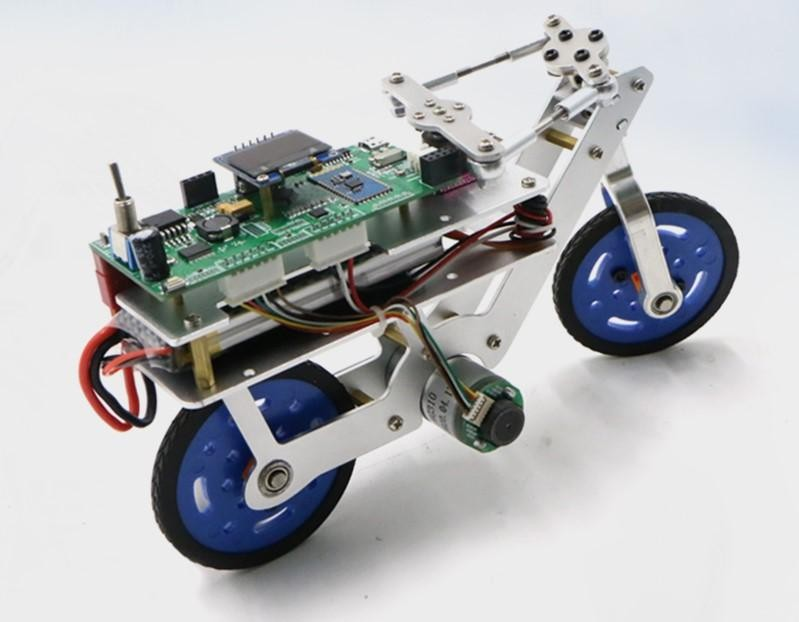
\includegraphics[width=0.7\linewidth]{figures/minibike/minibike}
	\caption{A picture for the MiniBike used in the experiments.}
	\label{fig:minibike}
\end{figure}


